\documentclass{utmreport}
\newcommand{\ReportTitle}{Vigenère Cipher over the Romanian Alphabet}
\newcommand{\ReportSubtitle}{\ReportCourse: Task 3.2, student number 12}
% Load after defining ReportTitle; optional per-report settings follow below.
% Shared identity and course details for all laboratory reports.
\student{Gafenco Victor}{FAF-241}
\supervisor{asist. univ. Zaica Maia}{}
\newcommand{\ReportCourse}{Cryptography}
\cityyear{Chișinău}{2026}
\institution{Technical University of Moldova}
\faculty{Faculty of Computers, Informatics, and Microelectronics}
\department{Department of Software Engineering}
\studyprogramme{Software Engineering Study Programme}
\newcommand{\repositoryurl}{https://github.com/yoda-dinmd/crypt-labs}

\providecommand{\ReportNumber}{\expandafter\ReportNumberFromJob\jobname\relax}
\def\ReportNumberFromJob#1#2#3#4\relax{#4}
\providecommand{\ReportSubtitle}{}
\selectlanguage{english}
\ifPDFTeX\else\setmonofont{Liberation Mono}\fi
\utmlogo{../latex/assets/UTM_Logo_English.jpeg}
\documenttype{Laboratory report no. \ReportNumber}
\reporttitle{\ReportTitle}
\reportsubtitle{\ReportSubtitle}
\hypersetup{
  pdftitle={\ReportTitle},
  pdfauthor={\UTMStudentName},
  pdfsubject={\ReportCourse{} laboratory report no. \ReportNumber}
}

% Shared wording for references to the supplied Cryptography handouts.
% Arguments: laboratory number, topic, optional descriptive text (including punctuation).
\newcommand{\ReportHandoutReference}[3]{%
  \textit{Laboratory Work No. #1. #2}. Supplied course handout#3}

\lstset{language=Java}
\begin{document}
\makeutmreporttitlepage
\tableofcontents
\clearpage
\begin{utmabstract}[Abstract]
This laboratory implements the Vigenère cipher for the 31-letter Romanian alphabet in Java. Student number 12 is even, so the assigned exercise is Task 3.2. A repeating keyword of at least seven letters controls modular addition for encryption and subtraction for decryption. The console validates inputs, removes message spaces, normalizes case and Romanian diacritics, and supports repeated operations. Reproducible console captures and automated tests demonstrate the implementation. The project integrates with the existing Maven parent and can be opened directly in IntelliJ IDEA.
\utmkeywords{Vigenère cipher, Romanian alphabet, polyalphabetic substitution, Java, Maven}
\end{utmabstract}

\utmintroduction
The objective is to implement Task 3.2 on page 7 of the supplied handout \cite{handout}. The task numbering differs from the theoretical section numbering: theoretical Section 3.1 describes Vigenère, whereas the even-numbered assignment is Task 3.2. Number 12 therefore requires Vigenère.

The application allows the user to select encryption or decryption, enter a key and a message or cryptogram, and obtain the result. This report follows the shared laboratory template and identity metadata used for the previous reports.

\chapter{Short theory}
\section{Alphabet and letter encoding}
The Romanian alphabet has 31 letters, with the following order and indices:
\begin{center}
\texttt{AĂÂBCDEFGHIÎJKLMNOPQRSȘTȚUVWXYZ}.
\end{center}
Thus $A=0$, $\text{Ă}=1$, $\text{Â}=2$, $B=3$, and $Z=30$. The cipher uses these indices, not Unicode character codes.

The handout requests 31 Romanian letters but also abbreviates the allowed ranges as A--Z and a--z. This implementation interprets the range as Romanian letters in either case, including Ă, Â, Î, Ș and Ț, consistent with the explicit 31-letter requirement. Ordinary message spaces are removed as required. Digits, punctuation and other characters are rejected with an explanation of the allowed alphabet.

\section{Repeating-key transformation}
For a normalized key of length $L\geq7$, position $i$ uses key index $k_{i\bmod L}$. Encryption and decryption are:
\begin{equation}
 c_i=(m_i+k_{i\bmod L})\bmod31,\qquad
 m_i=(c_i-k_{i\bmod L})\bmod31.
\end{equation}
The key repeats until the message ends. Repeated letters in the key are retained; unlike a keyword permutation, Vigenère uses every key position. A key longer than the message is valid, and only its required prefix is used. Spaces are removed before key alignment. Each new operation starts at the first key letter.

A fixed plaintext letter can produce different ciphertext letters at different key positions. This reduces the usefulness of a single frequency table, but repeating keys still expose periodic structure. Vigenère is a historical teaching cipher rather than a modern method for protecting confidential information. Decryption restores normalized letters; original capitalization and spaces cannot be recovered automatically.

\chapter{Implementation}
\section{Normalization and validation}
\texttt{VigenereCipher} owns the alphabet, validated key and transformations. NFC composition accepts decomposed Romanian diacritics, while cedilla variants Ş and Ţ map to Ș and Ț. Validation occurs before uppercase conversion to reject foreign characters such as ß that could otherwise expand into allowed letters.

Messages must contain at least one letter. Only ordinary spaces are discarded; tabs, line breaks, punctuation, digits and non-Romanian letters are rejected. Keys contain at least seven normalized letters and cannot contain spaces. Duplicate key letters count toward the minimum length because they represent distinct positions in the repeating sequence.

\section{Cipher implementation}
Both operations share the same loop. The direction of the shift is the only difference:
\begin{lstlisting}
String normalized = normalize(text, true);
StringBuilder result = new StringBuilder(normalized.length());
for (int i = 0; i < normalized.length(); i++) {
    int position = ALPHABET.indexOf(normalized.charAt(i));
    int shift = ALPHABET.indexOf(key.charAt(i % key.length()));
    int transformed = Math.floorMod(
            position + (decrypt ? -shift : shift), 31);
    result.append(ALPHABET.charAt(transformed));
}
\end{lstlisting}
\texttt{Math.floorMod} ensures that negative differences wrap to indices 0--30. Alphabet lookup has a fixed bound of 31 characters, so processing a message of length $n$ takes $O(n)$ time and $O(n)$ output space.

\section{Console and Maven integration}
\texttt{Main} provides options 1 (encrypt), 2 (decrypt) and 0 (exit). An invalid operation, key or message is requested again without discarding valid preceding fields. End of input exits cleanly. The console prints the normalized key and input to make alignment and formatting changes visible.

The \texttt{lab3} Maven module inherits Java 17 and plugin versions from the repository parent. Its executable JAR declares \texttt{md.utm.cryptography.lab3.Main} as the entry point. JUnit is used only for tests; the application has no external runtime dependencies. Open the root \texttt{pom.xml} in IntelliJ IDEA, select JDK 17, 21 or 25, and run this main class or Maven's \texttt{package} lifecycle.

\chapter{Results and verification}
\section{Worked Romanian example}
The message \texttt{Știința înseamnă putere} becomes \texttt{ȘTIINȚAÎNSEAMNĂPUTERE}, and the key is \texttt{CRIPTOGRAFIE}. The first seven transformations are shown below.
\begin{table}[htbp]
\centering
\caption{Initial positions of the Romanian Vigenère example}
\begin{tabular}{lrrrrrrr}\hline
Position & 0&1&2&3&4&5&6\\
Message index &22&23&10&10&16&24&0\\
Key index &4&20&10&18&23&17&8\\
Sum modulo 31 &26&12&20&28&8&10&8\\
Ciphertext &V&J&R&X&G&I&G\\\hline
\end{tabular}
\end{table}
The complete ciphertext is \texttt{VJRXGIGANXNEQDÎDOHLHE}. At position 11 the key restarts with C. Subtracting the same key sequence restores \texttt{ȘTIINȚAÎNSEAMNĂPUTERE}.

\section{Console evidence}
The following images render actual executable-JAR sessions captured through a pseudo-terminal, including echoed input. They are reproducible console captures rather than desktop screenshots. Adjacent text files preserve the raw transcripts. After building, regenerate them with:
\begin{lstlisting}[language={}]
python3 scripts/capture-results.py --lab lab3
\end{lstlisting}
\begin{figure}[htbp]
\centering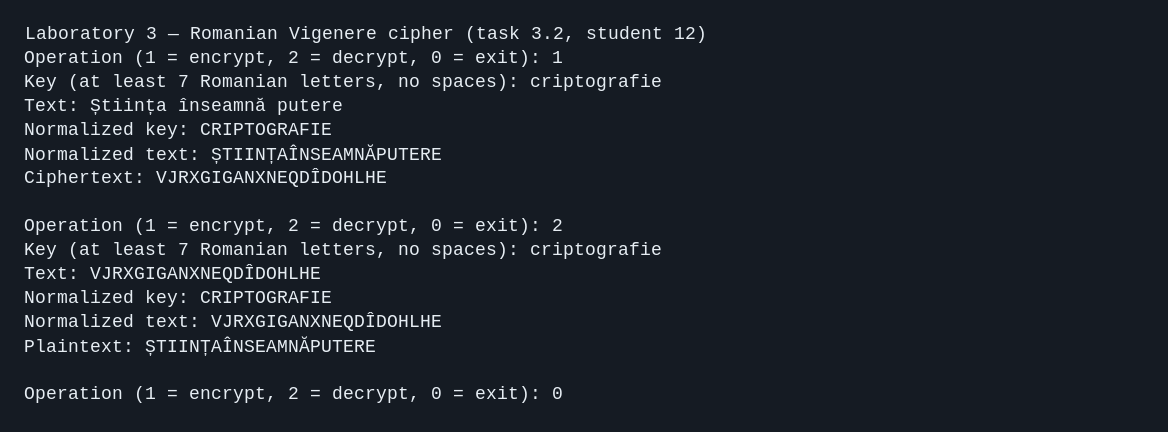
\includegraphics[width=\textwidth]{screenshots/roundtrip.png}
\caption{Romanian Vigenère encryption and decryption with the same key}
\end{figure}
\clearpage
The validation session rejects operation 3, a six-letter key, a key containing a space, and a message containing punctuation. Correcting each field completes encryption successfully.
\begin{figure}[htbp]
\centering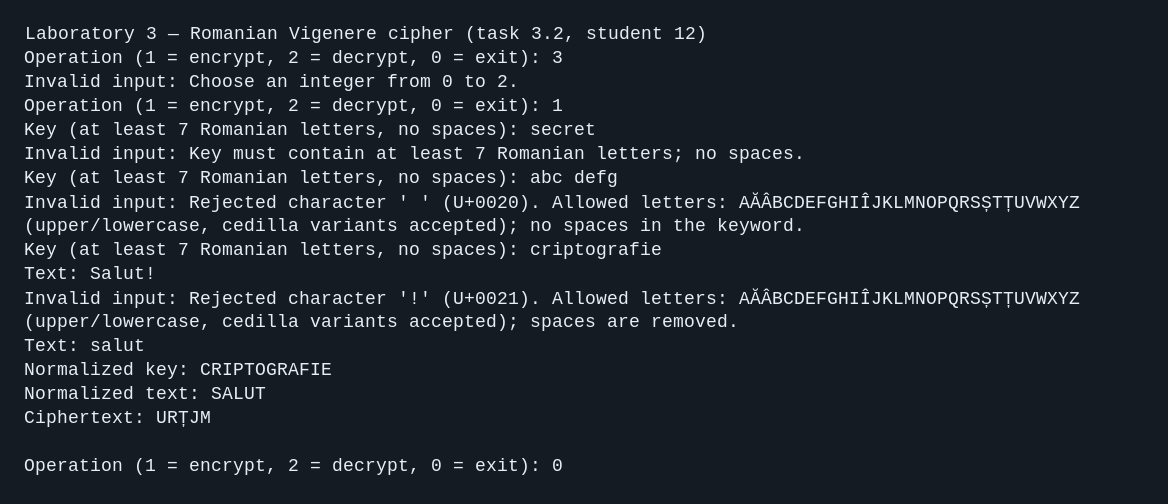
\includegraphics[width=\textwidth]{screenshots/invalid.png}
\caption{Input validation and successful recovery}
\end{figure}

\section{Automated verification}
Five JUnit tests cover the independently calculated Romanian example, exact alphabet order, all 31 letters at all 31 possible shifts, repeating-key alignment, key restart between calls, negative wraparound, and a key longer than the message. They also check lowercase and space normalization, composed and decomposed diacritics, cedilla variants, repeated-letter keys, and rejection of invalid keys and messages for both operations. The exhaustive shift check compares against alphabet rotations, testing 961 letter--shift combinations in each direction rather than relying only on round trips. The root Maven build also runs the existing Lab 1 tests.

\utmconclusions
Task 3.2 is implemented using a repeating key and modular arithmetic over the Romanian alphabet. The worked example and automated checks confirm that encryption and decryption are inverse operations for normalized input. Validation makes the permitted alphabet and minimum key length explicit. Compared with the Caesar cipher, the shift can change at each position, but repetition of the key remains a weakness. The exercise demonstrates polyalphabetic substitution and the importance of consistent encoding and normalization.

\chapter*{Source code and report materials}
\addcontentsline{toc}{chapter}{Source code and report materials}
The source, Maven module, tests and console evidence are in \texttt{lab3}. Shared metadata and the UTM class provide the report formatting. The compiled report is \path{reports/lab3.pdf}. The repository is available at \url{\repositoryurl}.
\end{document}
